\documentclass[10pt,twocolumn]{article}
\usepackage[margin=0.8in]{geometry}
\usepackage{amsmath,amssymb,booktabs,graphicx,xcolor,textcomp}
\usepackage{pgfplots}
\pgfplotsset{compat=1.17}
\usepackage[hidelinks]{hyperref}
\usepackage{caption}
\captionsetup{font=small,labelfont=bf}
% Generated by generate_tables.py -- do not edit by hand.
\newcommand{\ContrastRows}{$C_{\mathrm{DFS}}$ & $\Phi^+$ rise $-$ $\Psi^+$ rise, 0$\to$256\,ns & H2, H3 ($>0$) & +0.43 & [-0.13, +1.00] & 0.47\\
$C_{\mathrm{spec}}$ & rise with spectator in $|{+}\rangle$ $-$ in $|0\rangle$ & H1 ($>0$) & -0.20 & [-0.50, +0.11] & 0.53\\
$C_{\mathrm{stagger}}$ & $\Phi^+(256\,\mathrm{ns})-\Phi^+(0)$ & -- & +0.20 & [-0.22, +0.62] & 0.61\\
$C_{\mathrm{mem}}$ & DD32 $-$ echo at 16.384\,\textmu s & H3 ($>0$) & -0.14 & [-2.25, +1.97] & 0.89\\}
\newcommand{\ModelRows}{H0 & local & 5 & 10{,}420.9 & 10{,}436.6 & 5 & 100.3 & 115.05\\
H0\_1f & local & --- & --- & --- & 6 & 825.6 & 843.22\\
H3\_local & local & --- & --- & --- & 7 & 825.4 & 845.97\\
H1 & non-local & 6 & 2{,}482.6 & 2{,}501.4 & 6 & 97.6 & 115.27\\
H2 & non-local & 7 & 10{,}361.5 & 10{,}383.4 & 7 & 95.2 & 115.83\\
H3 & non-local & 8 & 148.6 & 173.7 & 8 & 825.4 & 848.92\\
Apparatus & non-local & 6 & 10{,}402.6 & 10{,}421.4 & 6 & 100.3 & 118.00\\}
\newcommand{\ValidationRows}{White (H0) & 100 & 0\% & 0\% & 0\% & 0\% & 0\%\\
Local $1/f$ & 100 & 100\% & 100\% & 100\% & 0\% & 0\%\\
Local $1/f$, Ramsey detuned & 100 & 100\% & 99\% & 96\% & 0\% & 0\%\\
Local OU memory & 100 & 100\% & 95\% & 95\% & 0\% & 0\%\\
Correlated Markovian (H2) & 50 & 0\% & 0\% & 0\% & 56\% & 56\%\\
Correlated OU, fast & 50 & 100\% & 100\% & 100\% & 44\% & 44\%\\
Correlated OU, slow & 50 & 100\% & 96\% & 96\% & 0\% & 0\%\\}
\newcommand{\StaggerPlots}{\addplot[blue!60!black,mark=*,mark size=1pt,thin] coordinates {(0,0.000) (16,0.674) (32,1.084) (48,0.781) (80,0.972) (160,1.216) (256,0.757)};
\addplot[blue!60!black,mark=*,mark size=1pt,thin] coordinates {(0,0.000) (16,0.976) (32,0.762) (48,0.976) (80,0.273) (160,0.332) (256,0.547)};
\addplot[blue!60!black,mark=*,mark size=1pt,thin] coordinates {(0,0.000) (16,0.025) (32,0.098) (48,0.538) (80,0.093) (160,-0.302) (256,0.445)};
\addplot[blue!60!black,mark=*,mark size=1pt,thin] coordinates {(0,0.000) (16,-0.893) (32,-0.019) (48,-0.429) (80,-0.141) (160,-0.542) (256,-0.176)};
\addplot[orange!80!black,mark=*,mark size=1pt,thin] coordinates {(0,0.000) (16,0.088) (32,-0.781) (48,0.015) (80,-0.425) (160,-0.591) (256,0.156)};
\addplot[orange!80!black,mark=*,mark size=1pt,thin] coordinates {(0,0.000) (16,0.346) (32,0.932) (48,0.571) (80,0.644) (160,0.820) (256,1.142)};
\addplot[orange!80!black,mark=*,mark size=1pt,thin] coordinates {(0,0.000) (16,0.122) (32,0.044) (48,-0.039) (80,-0.279) (160,0.664) (256,-0.171)};
\addplot[orange!80!black,mark=*,mark size=1pt,thin] coordinates {(0,0.000) (16,-0.166) (32,0.600) (48,0.166) (80,-0.591) (160,0.561) (256,0.264)};
\addplot[orange!80!black,mark=*,mark size=1pt,thin] coordinates {(0,0.000) (16,-0.786) (32,-0.723) (48,-0.762) (80,-0.288) (160,-0.600) (256,-1.001)};
\addplot[orange!80!black,mark=*,mark size=1pt,thin] coordinates {(0,0.000) (16,-0.025) (32,0.449) (48,-0.567) (80,0.210) (160,-0.308) (256,0.068)};}
\newcommand{\JobId}{dbtp67dav06s73cfbsm0}
\newcommand{\Blocks}{5}
\newcommand{\Shots}{2{,}048}
\newcommand{\TotalShots}{499{,}712}
\newcommand{\QpuSeconds}{139}
\newcommand{\AARaw}{1.15}
\newcommand{\SFortyEight}{0.62}
\newcommand{\LockedDBIC}{10{,}263}
\newcommand{\HoRmseHZero}{0.130}
\newcommand{\HoRmseHThree}{0.143}
\newcommand{\HoT}{-0.24}
\newcommand{\HoP}{0.82}
\newcommand{\LockSha}{38ebfe7f7c007633281039bca551af963e8335db54e6e6915a1e3f5be4a64fd8}
\newcommand{\QpySha}{158de03260c429c8170cd3e3b296ade8045881e385370f1774619344e57b9da1}
\newcommand{\AmendSha}{7fb094d7a347496527db32d6a2b668a0723e7806cb5cefdb35ce7129e40a6947}


\title{\bfseries No evidence of spatially correlated or non-Markovian dephasing across ten
couplers of \texttt{ibm\_marrakesh} --- and why a white-noise null is not enough to look for it}
\author{Devin Phillip Davis\\ \small Agile Defense Systems LLC}
\date{20 November 2026 \quad (CORRELATED-NOISE-01 Stage 1 results, version 1.0)}

\begin{document}
\maketitle

\begin{abstract}
\noindent
We report Stage~1 of a preregistered hardware test for non-local dephasing on a 156-qubit IBM
Heron~r2 processor. Ten couplers at least five hops apart were measured simultaneously in every
circuit (one job, \TotalShots{} circuit shots, \QpuSeconds{}\,s of QPU time): Bell states under
dynamical decoupling with sub-slot sublattice staggers from 0 to 256\,ns, $\Phi^+$ versus $\Psi^+$,
active versus idle spectators, echo and DD pulse-count series, and Ramsey arms. Spatially correlated
dephasing predicts that staggering helps $\Phi^+$ and hurts $\Psi^+$ equally; we see no such
asymmetry ($C_{\mathrm{DFS}}=+0.43$\,pp, 95\% CI $[-0.13,+1.00]$), no spectator effect, no
memory contrast and no pulse-collision step. The analysis as locked selects a non-Markovian
memory model (H3) over white noise by $\Delta\mathrm{BIC}=\LockedDBIC$ but fails its preregistered
held-out test ($p=\HoP$), so the transferable memory claim is falsified under its own kill
criterion. A validation on synthetic counts shows why the in-sample selection is uninformative: with
white noise as the only null, the locked analysis selects H3 in 100\% of replicates of purely local
$1/f$ or Ornstein--Uhlenbeck noise. An amended analysis with local coloured-noise nulls (recorded
before the job but published after it) selects the local model and reaches the same verdict: local
noise only. The result bounds fast correlated dephasing at the 1\,pp level and says nothing about
correlations slower than about 1\,\textmu s.
\end{abstract}

\section{Question and models}
Can Bell-state measurements on pairs of transmons distinguish spatially correlated or temporally
non-Markovian dephasing from independent local noise, spectator $ZZ$ coupling and classical control
artefacts? Five models were fitted to the same data:
\textbf{H0}, independent local amplitude damping and white dephasing;
\textbf{H1}, H0 plus static spectator $ZZ$;
\textbf{H2}, H0 plus spatially correlated Markovian dephasing;
\textbf{H3}, a coloured (Ornstein--Uhlenbeck) bath with a spatial correlation $C_{uv}$; and
\textbf{Apparatus}, finite-width pulse collisions between overlapping drive envelopes.

Under DD with $N$ pulses over $T=8.192$\,\textmu s, offsetting one sublattice by $\Delta$ changes
the pair's toggling-frame overlap $\alpha_{uv}=1-2\Delta/\tau_{\mathrm{slot}}$. For correlated
dephasing $\gamma_{uv}$ the decay rates are
$\Gamma_{\Phi^\pm}=\gamma_u+\gamma_v+2\alpha_{uv}\gamma_{uv}$ and
$\Gamma_{\Psi^\pm}=\gamma_u+\gamma_v-2\alpha_{uv}\gamma_{uv}$, so staggering raises $\Phi^+$ and lowers
$\Psi^+$ by equal amounts. Local noise moves both alike~\cite{tripathi,pazsilva,sung}. Spectator $ZZ$ shows up only when the
spectator is in $|{+}\rangle$; pulse collisions give a step that is complete by $\Delta=48$\,ns.

\section{Design}
\paragraph{Cohort.} Ten couplers were chosen by a fixed rule on the lock-time calibration
(pairwise distance $\ge5$ hops, lowest CZ error): four for training and six held out. All ten run in
every PUB, so the held-out test costs no extra circuits and shares the same drift.

\paragraph{Conditions.} Echo ($N=1$) at 2, 4, 8, 16\,\textmu s; DD with $N=8,16,32$ at 8.192\,\textmu s
and $N=32$ at 16.384\,\textmu s; $\Phi^+$ under DD16 at offsets 0, 16, 32, 48, 80, 160, 256\,ns;
$\Psi^+$ at 0 and 256\,ns; $\Phi^+$ with the spectator in $|{+}\rangle$ at 0 and 256\,ns; Ramsey at 2--16\,\textmu s;
a duplicated 0\,ns $\Phi^+$ circuit per block as an A/A sentinel; and two-qubit readout calibration.
Bell fidelity comes from three Pauli bases.

\paragraph{Size.} Amendment A-2 (before the job) reduced the preregistered 8 blocks $\times$ 4{,}200
shots to \Blocks{} blocks $\times$ \Shots{} shots (244 PUBs) to fit the IBM Open Plan quota.

\paragraph{Decision rules (as locked).} GLS fit on the training couplers; a model is selected if it
beats H0 by $\Delta\mathrm{BIC}\ge8$. Four mechanistic contrasts across all ten couplers (df~$=9$,
Holm). Kill criterion: if H1, H2 or H3 wins in-sample but does not beat H0 on held-out RMSE
(paired $t$, df~$=5$), ``the transferable quantum-control claim is falsified''. Stage~2, a replication
on \texttt{ibm\_fez}, runs only if Stage~1 passes.

\section{Why the locked analysis needed an amendment}
Before the job we ran both analyses on synthetic count sets built in the locked bit layout, with
lock-time $T_1$ values, per-qubit readout error, block drift and \Shots{}-shot sampling
(Table~\ref{tab:validation}). The locked analysis selected H3, the ``memory'' model, on 100\% of
replicates whose truth was \emph{independent local} $1/f$ or OU noise, and opened the Stage-2 gate on
95--100\% of them. Three causes: white noise is the only null, so any coloured local noise that
decays differently under Ramsey, echo and DD favours H3; the held-out test calibrates H0 and H3 from
different arms; and single-quadrature Ramsey arms turn a frame detuning into apparent decay.

Amendment A-3 adds two local nulls (H0\_1f, independent $1/f$ plus a white floor; H3\_local, H3
without spatial correlation), requires a non-local model to beat the \emph{best local} model by
$\Delta\mathrm{BIC}\ge8$, drops the Ramsey arms from the fit, calibrates every model from the same
echo-DD32 arm, scores the held-out couplers on the change in $\Phi^+$ with stagger (the preregistered
target), and draws the training split from a generator seeded by the QPY hash. Circuits, schedule,
cohort and size are unchanged. On the same synthetic data A-3 made no non-local claim on any of 400
local-noise replicates, and confirmed fast correlated dephasing in 44--56\% of replicates; its power
target of 80\% was not met.

\paragraph{Provenance of A-3.} The A-3 record (SHA-256 \texttt{\detokenize{7fb094d7...}}) hashes the
lock, the QPY, the analysis code and the validation, and was written at 23:02\,UTC on 16 November,
32 minutes before the job was created. It was not committed or pushed until after the job, and the job
was submitted from a checkout whose runner ran only the locked analysis. The evidence that A-3
predates the data is therefore local and cannot be checked independently; readers who do not accept
it should treat A-3 as post hoc. We report both analyses. They reach the same verdict.

\begin{table*}[t]
\centering\small
\caption{Validation on synthetic counts (before the job). ``Locked'' columns: how often the locked
analysis selects H3, opens the Stage-2 gate, and makes the H3 memory claim. ``A-3'' columns: any
non-local claim, and correlated dephasing supported.}
\label{tab:validation}
\begin{tabular}{@{}lrrrrrr@{}}
\toprule
& & \multicolumn{3}{c}{Locked analysis} & \multicolumn{2}{c}{A-3}\\
\cmidrule(lr){3-5}\cmidrule(l){6-7}
Truth & Replicates & H3 selected & Stage-2 gate & H3 claim & Non-local claim & Corr.\ dephasing\\
\midrule
\ValidationRows
\bottomrule
\end{tabular}
\end{table*}

\section{Results}
Job \texttt{\JobId} ran on 16 November 2026 (\QpuSeconds{}\,s charged). The saved counts were
re-queried and match IBM's stored result for all 244 PUBs.

\paragraph{Mechanistic contrasts.} None is significant (Table~\ref{tab:contrasts}). $\Phi^+$ is flat
across the offsets to within 0.25\,pp (Fig.~\ref{fig:stagger}). $C_{\mathrm{DFS}}$'s interval excludes
the 1.4--3.0\,pp asymmetries that the validation produced for fast correlated dephasing. The step
fraction $S_{48}=\SFortyEight$ is below the 0.75 the Apparatus model needs, and with a 0.2\,pp total
rise it is mostly noise. The A/A sentinel's RMS difference was \AARaw\,pp, matching the 1.0--1.1\,pp
drift floor measured in earlier runs on this device.

\begin{table*}[t]
\centering\small
\caption{Mechanistic contrasts, mean over 10 couplers in percentage points (df~$=9$, Holm across
four). Identical in both analyses.}
\label{tab:contrasts}
\begin{tabular}{@{}lllrcr@{}}
\toprule
Contrast & Definition & Needed for & Mean (pp) & 95\% CI (pp) & Holm $p$\\
\midrule
\ContrastRows
\bottomrule
\end{tabular}
\end{table*}

\begin{table}[t]
\centering\small
\caption{Model selection on the training couplers. Locked analysis: 23 conditions, lowest-CZ-error
split. A-3: 19 conditions (no Ramsey), hash-seeded split.}
\label{tab:models}
\setlength{\tabcolsep}{3pt}
\begin{tabular}{@{}llrrrrrr@{}}
\toprule
& & \multicolumn{3}{c}{Locked} & \multicolumn{3}{c}{A-3}\\
\cmidrule(lr){3-5}\cmidrule(l){6-8}
Model & Type & $k$ & $\chi^2$ & BIC & $k$ & $\chi^2$ & BIC\\
\midrule
\ModelRows
\bottomrule
\end{tabular}
\end{table}

\begin{figure}[t]
\centering
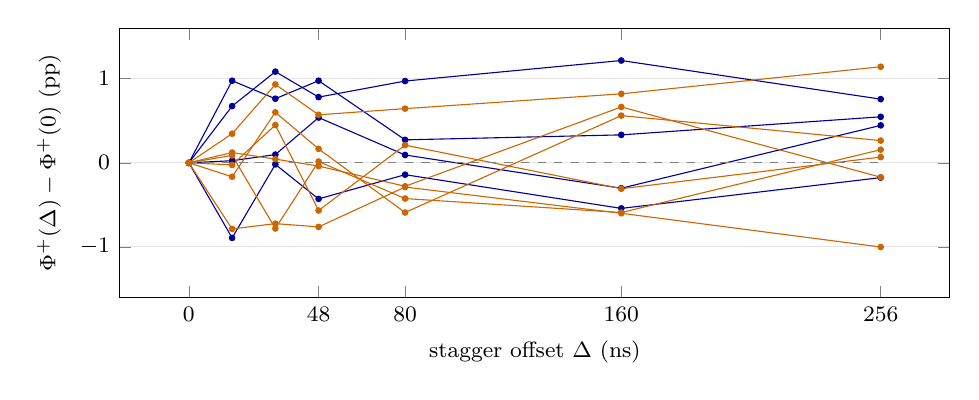
\begin{tikzpicture}
\begin{axis}[width=\columnwidth,height=5cm,xlabel={stagger offset $\Delta$ (ns)},
  ylabel={$\Phi^+(\Delta)-\Phi^+(0)$ (pp)},xtick={0,48,80,160,256},ymin=-1.6,ymax=1.6,
  tick label style={font=\footnotesize},label style={font=\footnotesize},ymajorgrids,grid style={gray!20}]
\StaggerPlots
\addplot[gray,dashed,domain=0:256] {0};
\end{axis}
\end{tikzpicture}
\caption{Change in raw $\Phi^+$ Bell fidelity with stagger offset under DD16, per coupler (blue:
locked training couplers; orange: held out). Correlated dephasing at the strengths simulated in
the validation would raise every curve by 1.4--3\,pp at 256\,ns.}
\label{fig:stagger}
\end{figure}

\paragraph{Analysis as locked.} H3 is selected by $\Delta\mathrm{BIC}=\LockedDBIC$ over H0
(Table~\ref{tab:models}), with two of its parameters at their bounds. On the six held-out couplers its
mean RMSE is \HoRmseHThree{} against \HoRmseHZero{} for H0 (paired $t_5=\HoT$, $p=\HoP$). Under the
preregistered kill criterion the transferable H3 claim is \emph{falsified}. Given the validation,
the in-sample selection carries no information about spatial correlation either way.

\paragraph{Amendment A-3.} H0 is the best local model and no non-local model beats it (the closest,
H1, is 0.22 BIC behind). Decision: \emph{local noise only}. ``Local non-white dephasing'' is not
reported because H0\_1f does not beat H0. A post-hoc diagnostic showed that H0\_1f, H3\_local and H3
fit worse than H0 although each contains it, because their white-floor bound (40\,kHz) sits below the
fitted 57\,kHz; raising the bound makes all three collapse onto H0 and changes no decision.

\paragraph{Descriptive.} Ramsey decays much faster than echo and varies widely between couplers (0.18--0.90
at 16\,\textmu s against 0.82--0.95 for echo), consistent with low-frequency local noise, a frame
detuning, or both; one quadrature cannot tell them apart. One coupler, (1,2), had a two-qubit readout
assignment fidelity of 0.89; the other nine were 0.95--0.98.

\section{What this shows}
\begin{itemize}\itemsep0pt
\item \textbf{Fast correlated dephasing} (faster than the 512\,ns DD slot): not seen, bounded below
about 1\,pp of $\Phi^+/\Psi^+$ asymmetry.
\item \textbf{Slow correlated noise} (correlation time above about 1\,\textmu s): not tested; DD16
refocuses it and its expected asymmetry is below 0.1\,pp.
\item \textbf{Spectator $ZZ$ and pulse collisions}: not seen.
\item \textbf{Correlated memory}: not seen, but $C_{\mathrm{mem}}$'s interval is wide ($\pm2$\,pp).
\item Stage~2 on \texttt{ibm\_fez} does not run.
\end{itemize}

The methodological point generalises beyond this device. A model-selection test for bath memory or
spatial correlation needs local coloured-noise nulls; with white noise as the only null, ordinary
$1/f$ noise, which every superconducting qubit has, is enough to select a ``non-Markovian'' model by
thousands of BIC units. We recommend that validation on synthetic local coloured noise be part of any
such preregistration.

\paragraph{Limitations.} One job, one device, ten couplers, five blocks. The held-out test's power is
limited (44--56\% on simulated fast correlated truths). A-3 was not public before the data.

\section*{Data and code availability}
The accompanying record contains the preregistration, theory and identifiability notes, amendments
A-2 and A-3 with the A-3 validation, the lock file (\texttt{\detokenize{38ebfe7f...}}), the compiled QPY
(\texttt{\detokenize{158de032...}}), the raw counts for all 244 PUBs, both analysis outputs, the bound
diagnostic and the scripts that produce every table and figure, with a SHA-256 manifest. Two IBM Cloud
account identifiers were removed from the raw-counts file; no count was changed. Source repository:
\url{https://github.com/quantum-osiris/osiris-cli} (\texttt{docs/phase3/}, \texttt{phase2/correlated\_noise\_01/}).

\section*{Acknowledgements}
We acknowledge the use of IBM Quantum services; the views expressed are the author's and do not
reflect the official policy or position of IBM or the IBM Quantum team. Analysis code and this
manuscript were prepared with the assistance of AI coding tools under the author's direction and
review.

\begin{thebibliography}{9}\small
\bibitem{tripathi} V.~Tripathi \emph{et al.}, ``Suppression of crosstalk in superconducting qubits
using dynamical decoupling,'' \emph{Phys.\ Rev.\ Applied} \textbf{18}, 024068 (2022).
\bibitem{pazsilva} G.~A.~Paz-Silva \emph{et al.}, ``Multiqubit spectroscopy of Gaussian quantum noise,''
\emph{Phys.\ Rev.\ A} \textbf{95}, 022121 (2017).
\bibitem{sung} Y.~Sung \emph{et al.}, ``Multi-level quantum noise spectroscopy,''
\emph{Nat.\ Commun.} \textbf{12}, 967 (2021).
\end{thebibliography}
\end{document}
